\documentclass[a4paper, 14pt]{extarticle}
\usepackage{geometry}

\usepackage{cmap} % Улучшенный поиск русских слов в полученном pdf-файле
\usepackage{mathtext} % русские буквы в формулах
\defaulthyphenchar=127 % Если стоит до fontenc, то переносы не впишутся в выделяемый текст при 
%копировании его в буфер обмена
\usepackage[T2A]{fontenc}
\usepackage[utf8]{inputenc}
\usepackage[english, russian]{babel}
%\usepackage{pscyr}  
%\renewcommand{\rmdefault}{ftm} % ftm - (TimesNewRoman), fac - Academy, fad - Advertisement, flz - 
%Lazurski, fcr - CourierNewPSM, others in pscyr.sty

\usepackage{amsthm,amsfonts,amsmath,amssymb,amscd} % Математические дополнения от AMS
\usepackage{mathtools} % Добавляет окружение multlined

\usepackage{longtable} % Длинные таблицы
\usepackage{multirow,makecell,array} % Улучшенное форматирование таблиц
%\usepackage{booktabs} % Возможность оформления таблиц в классическом книжном стиле

\usepackage{soulutf8} % Поддержка переносоустойчивых подчёркиваний и зачёркиваний
\usepackage{icomma} % Запятая в десятичных дробях

\usepackage[usenames,dvipsnames,svgnames,table,rgb]{xcolor}

\usepackage{hyperref}

\usepackage{graphicx} % Подключаем пакет работы с графикой
\graphicspath{{../images/}{images/}} % Пути к изображениям

%%% Подписи %%%
\usepackage[singlelinecheck=off,center]{caption}
\usepackage{subcaption}

\usepackage[onehalfspacing]{setspace}

%%% Списки %%%
\usepackage{enumitem}

%%% Библиография %%%
\usepackage{cite} % Красивые ссылки на литературу

%%% Оглавление %%%
\usepackage[nottoc]{tocbibind}
\usepackage{tocloft}
\usepackage{titlesec}

\usepackage{titlesec} % Растояние между заголовками и текстом
\usepackage{float}
\usepackage{listings} % Listings
\usepackage{minted}

\usepackage{lipsum}

%\usepackage[linesnumbered,ruled,vlined]{algorithm2e}

\geometry{a4paper,top=2cm,bottom=2cm,left=2cm,right=1cm}
%%% Выравнивание и переносы %%%
\sloppy                             % Избавляемся от переполнений
\clubpenalty=10000                  % Запрещаем разрыв страницы после первой строки абзаца
\widowpenalty=10000                 % Запрещаем разрыв страницы после последней строки абзаца
\usepackage{indentfirst}
\frenchspacing
\setlength{\parindent}{2.5em} % Абзацный отступ
\linespread{1.3}

% colors
\definecolor{linkcolor}{rgb}{0.9,0,0}
\definecolor{citecolor}{rgb}{0,0.6,0}
\definecolor{urlcolor}{rgb}{0,0,1}
\definecolor{mygreen}{rgb}{0,0.6,0}
\definecolor{mygray}{rgb}{0.5,0.5,0.5}
\definecolor{mymauve}{rgb}{0.58,0,0.82}
\definecolor{myblack}{rgb}{0,0,0}

\hypersetup{				% Гиперссылки
    unicode=true,          % non-Latin characters in Acrobat’s bookmarks
    pdftoolbar=true,        % show Acrobat’s toolbar?
    pdfmenubar=true,        % show Acrobat’s menu?
    pdffitwindow=false,     % window fit to page when opened
    pdfstartview={FitH},    % fits the width of the page to the window
    pdftitle={Classification and Aggregation of News Articles Using Methods and Models of Natural Language Processing},    % title
    pdfauthor={Vasily Vdovkin},     % author
    pdfsubject={Course work},   % subject of the document
    pdfcreator={Vasily Vdovkin},   % creator of the document
    pdfproducer={Vasily Vdovkin}, % producer of the document
    pdfkeywords={nlp}{text}{clusterization}{aggregation}{news}{articles}{svm}{rnn}{deep}{learning}, % Ключевые слова
    pdfnewwindow=true,
    pdflang={ru},
    linktocpage=true,
    plainpages=false,
    colorlinks,       	    % false: ссылки в рамках; true: цветные ссылки
    linkcolor={linkcolor},      % цвет ссылок типа ref, eqref и подобных
    citecolor={citecolor},      % цвет ссылок-цитат
    urlcolor={urlcolor},        % цвет гиперссылок
}

%% Рисунки %%%
\DeclareCaptionLabelSeparator{emdash}{. }
\captionsetup[figure]{labelsep=emdash,font=onehalfspacing,position=bottom}
\captionsetup[subfigure]{subrefformat=simple,labelformat=simple}
\renewcommand\thesubfigure{(\alph{subfigure})}

\captionsetup{%
    singlelinecheck=off,                % Многострочные подписи, например у таблиц
    skip=2pt,                           % Вертикальная отбивка между подписью и содержимым рисунка или таблицы определяется ключом
    justification=centering,            % Центрирование подписей, заданных командой \caption
}

%% Подписи подрисунков %%%
\renewcommand{\thesubfigure}{\asbuk{subfigure}}           % Буквенные номера подрисунков
\captionsetup[subfigure]{font={normalsize},               % Шрифт подписи названий подрисунков (не отличается от основного)
    labelformat=brace,                                    % Формат обозначения подрисунка
    justification=centering,                              % Выключка подписей (форматирование), один из вариантов            
}

%%% Списки %%%
% Используем короткое тире (endash) для ненумерованных списков (ГОСТ 2.105-95, пункт 4.1.7, требует дефиса, но так лучше смотрится)
\renewcommand{\labelitemi}{\normalfont\bfseries{--}}

% Перечисление строчными буквами русского алфавита (ГОСТ 2.105-95, 4.1.7)
%\makeatletter
%    \AddEnumerateCounter{\asbuk}{\russian@alph}{щ}
%\makeatother
%\setlist[enumerate,1]{label=\asbuk{enumi})} % первого уровня 1), 2)...
%\setlist[enumerate,2]{label=\arabic*)} % второго уровня а), б) ... 

\setlist{nosep,%                                    % Единый стиль для всех списков (пакет enumitem), без дополнительных интервалов.
    labelindent=\parindent,leftmargin=*%            % Каждый пункт, подпункт и перечисление записывают с абзацного отступа
}

%%% Переопределение именований %%%
\addto\captionsrussian{%
    \renewcommand{\partname}{Часть}
    \renewcommand{\abstractname}{Аннотация}
    \renewcommand{\contentsname}{Содержание} % (ГОСТ Р 7.0.11-2011, 4)
    \renewcommand{\figurename}{Рис.} % (ГОСТ Р 7.0.11-2011, 5.3.9)
    \renewcommand{\tablename}{Таблица} % (ГОСТ Р 7.0.11-2011, 5.3.10)
    \renewcommand{\indexname}{Предметный указатель}
    \renewcommand{\listfigurename}{Список рисунков}
    \renewcommand{\listtablename}{Список таблиц}
}
%
%%% Старт отсчет страниц с титульника
\makeatletter
\renewenvironment{titlepage}
 {%
  \if@twocolumn
    \@restonecoltrue\onecolumn
  \else
    \@restonecolfalse\newpage
  \fi
  \thispagestyle{empty}%
 }
 {%
  \if@restonecol
    \twocolumn
  \else
    \newpage
  \fi
 }
\makeatother
%%%

%%% Библиография %%%
\makeatletter
\bibliographystyle{utf8gost71u}     % Оформляем библиографию по ГОСТ 7.1 (ГОСТ Р 7.0.11-2011, 5.6.7)
\renewcommand{\@biblabel}[1]{#1.}   % Заменяем библиографию с квадратных скобок на точку
\makeatother

%%% Оглавление %%%
\cftsetrmarg{2.55em plus1fil} %To have the (sectional) titles in the ToC, etc., typeset ragged right with no hyphenation
\renewcommand{\cftsecdotsep}{\cftdotsep} % отбивка точками до номера страницы начала главы/раздела
\renewcommand{\cftsecpagefont}{\normalfont}        % нежирные номера страниц у глав в оглавлении
\renewcommand{\cftsecleader}{\cftdotfill{\cftsecdotsep}}% нежирные точки до номеров страниц у глав в оглавлении
\renewcommand{\cfttoctitlefont}{\filright\fontsize{16pt}{18pt}\selectfont\bfseries} % Размер заголовка оглавления

%\renewcommand{\cftsecfont}{}                       % нежирные названия глав в оглавлении
%\renewcommand\cftsecaftersnum{.\ }   % добавляет точку с пробелом после номера раздела в оглавлении
%\renewcommand\cftsecaftersnum{.\ }    % добавляет точку с пробелом после номера подраздела в оглавлении
%\renewcommand\cftsubsecaftersnum{.\ } % добавляет точку с пробелом после номера подподраздела в оглавлении
%\renewcommand\cftsecaftersnum{\quad}     % добавляет \quad после номера раздела в оглавлении
%\renewcommand\cftsecaftersnum{\quad}      % добавляет \quad после номера подраздела в оглавлении
%\renewcommand\cftsubsecaftersnum{\quad}   % добавляет \quad после номера подподраздела в оглавлении
%\addtocontents{toc}{~\hfill{Стр.}\par}% добавить Стр. над номерами страниц

%%% Оформление заголовков глав, разделов, подразделов %%%
\titleformat{\section}[block]
    %{\filcenter\fontsize{16pt}{18pt}\selectfont\bfseries}{\thesection\cftsecaftersnum}{0.5em}{} % по центру
    {\filright\fontsize{16pt}{18pt}\selectfont\bfseries}{\thesection\cftsecaftersnum}{0.5em}{} % справа

\titleformat{\subsection}[block]
    %{\filcenter\fontsize{16pt}{18pt}\selectfont\bfseries}{\thesubsection\cftsubsecaftersnum}{0.5em}{}
    {\filright\fontsize{16pt}{18pt}\selectfont\bfseries}{\thesubsection\cftsubsecaftersnum}{0.5em}{}

\titleformat{\subsubsection}[block]
    %{\filcenter\fontsize{16pt}{18pt}\selectfont\bfseries}{\thesubsubsection\cftsubsecaftersnum}{0.5em}{}
    {\filright\fontsize{16pt}{18pt}\selectfont\bfseries}{\thesubsubsection\cftsubsecaftersnum}{0.5em}{}

%\renewcommand{\abstractnamefont}{\fontsize{16pt}{18pt}\selectfont\bfseries} % Размер заголовка аннтоации


% Расстояние между текстом и заголовками
%\setlength{\abstitleskip}{-25pt} % расстояние между заголовком аннтоации и тестом
\titlespacing{\section}{\parindent}{*2}{*1} % Расстояние между заголовком раздела и текстом должно быть равно удвоенному межстрочному интервалу.  Расстояние между основаниями строк заголовка принимают такими же, как в тексте
\titlespacing{\subsection}{\parindent}{*2}{*1}
\titlespacing{\subsubsection}{\parindent}{*2}{*1}

% Listings
\captionsetup[lstlisting]{labelsep=emdash}
\lstset{ %
  backgroundcolor=\color{white},   % choose the background color; you must add \usepackage{color} or \usepackage{xcolor}
  basicstyle=\ttfamily\footnotesize,        % the size of the fonts that are used for the code
  breakatwhitespace=false,         % sets if automatic breaks should only happen at whitespace
  breaklines=true,                 % sets automatic line breaking
  captionpos=t,                    % sets the caption-position to bottom
  commentstyle=\ttfamily,    % comment style
  columns=fixed,
  deletekeywords={...},            % if you want to delete keywords from the given language
  escapeinside={\%*}{*)},          % if you want to add LaTeX within your code
  extendedchars=true,              % lets you use non-ASCII characters; for 8-bits encodings only, does not work with UTF-8
  frame=none,	                   % adds a frame around the code
  keepspaces=true,                 % keeps spaces in text, useful for keeping indentation of code (possibly needs columns=flexible)
  keywordstyle=\ttfamily\bfseries,       % keyword style
  otherkeywords={*,...},           % if you want to add more keywords to the set
  numbers=left,                    % where to put the line-numbers; possible values are (none, left, right)
  numbersep=5pt,                   % how far the line-numbers are from the code
  numberstyle=\footnotesize\color{mygray}, % the style that is used for the line-numbers
  rulecolor=\color{black},         % if not set, the frame-color may be changed on line-breaks within not-black text (e.g. comments (green here))
  showspaces=false,                % show spaces everywhere adding particular underscores; it overrides 'showstringspaces'
  showstringspaces=false,          % underline spaces within strings only
  showtabs=false,                  % show tabs within strings adding particular underscores
  stepnumber=1,                    % the step between two line-numbers. If it's 1, each line will be numbered
  stringstyle=\ttfamily,     % string literal style
  tabsize=4,	                   % sets default tabsize to 2 spaces
  title=\lstname                   % show the filename of files included with \lstinputlisting; also try caption instead of title
  % stringstyle=\color{mymauve}\ttfamily,     % string literal style
  % keywordstyle=\ttfamily\color{blue},       % keyword style
  % commentstyle=\ttfamily\color{mygreen},    % comment style
} % Файл со стилями

\makeatletter
\setlength{\@fptop}{0pt}
\makeatother
%

\begin{document}

\begin{titlepage}
	\begin{center}
		ФЕДЕРАЛЬНОЕ ГОСУДАРСТВЕННОЕ АВТОНОМНОЕ
		
		ОБРАЗОВАТЕЛЬНОЕ УЧРЕЖДЕНИЕ ВЫСШЕГО ОБРАЗОВАНИЯ
		
		<<НАЦИОНАЛЬНЫЙ ИССЛЕДОВАТЕЛЬСКИЙ УНИВЕРСИТЕТ
		
		<<ВЫСШАЯ~ШКОЛА~ЭКОНОМИКИ>>
		\vspace{1cm}
		
		МОСКОВСКИЙ ИНСТИТУТ ЭЛЕКТРОНИКИ И МАТЕМАТИКИ\\  
		им. А.Н. ТИХОНОВА
		\vspace{1cm}
		
		Вдовкин Василий Алексеевич, группа БИВ-144
		
		\vspace{1cm}
		
		\MakeUppercase{\textbf{Методы сокращения текста и извлечения ключевой информации из русскоязычных новостных статей}}
		
		\vspace{1cm}
		
		Выпускная квалификационная работа 
		
		по направлению 09.03.01 Информатика и вычислительная техника 
		
		студентов образовательной программы бакалавриата
		
		<<Информатика и вычислительная техника>>
		
	\end{center}
  	\vspace{1cm}
  	\begin{flushright}
  		Студент~\rule{4cm}{.1pt}~В.А.\,Вдовкин
  	\end{flushright}
  	\vspace{1cm}
  	\begin{flushleft}
  		Рецензент \hfill  Руководитель
  		
  		к.т.н., доцент \hfill старший преподаватель
  		
  		?.?. ???? \hfill Ф.В.\,Волкова
  		
  		\rule{4cm}{.1pt} \hfill \rule{4cm}{.1pt}
  		
  	\end{flushleft}
  	\vfill\center{Москва 2018 г.}
\end{titlepage} % Титульник
\titleformat{\section}[block]
{\centering\fontsize{16pt}{18pt}\selectfont\bfseries}{\thesection\cftsecaftersnum}{0.5em}{} % по центру

\section*{Аннотация}
Данная работа описывает процесс реализации сервиса, способного значительно улучшить
и упростить пользовательское взаимодействие с новостным контентом, используя обработку
естественного языка (Natural Language Processing, NLP). Сервис анализирует поток русскоязычных новостных статей в реальном времени, группирует их по конкретным событиям и выделяет ключевую информацию о событии.
Для построения такого сервиса мы изучаем и используем различные методы и модели, распространенные в NLP для решения следующих задач:
нормализация, векторизация, кластеризация и суммаризация текста.
Кластеризация используется для выделения из потока данных множества статей, относящемся к одному событию.
Мы собираем и обрабатываем большое количество данных с web-сайтов медиа и обучаем векторизатор TF-IDF, позволяющий использовать K-means для кластеризации.
Суммаризация извлекает самые информативные предложения из кластера-события и формирует параграф из 5 следующих по смыслу предложений. Для суммаризации используются две модели: SimBasic и DivRank. Выбранные решения сравниваются и оцениваются.


\section*{Abstract}
This work describes implementation of the service that can significantly improve user experience in news content consumption by using Natural Language Processing (NLP for short). This service analyses stream of news articles from russian media web-sites in real-time, groups news by events and extracts the most valuable information about the events.
To implement this service we first research and then use models and methods from NLP to find suitable solution for the following problems: normalization, vectorization, clusterization and summarization of text.
Clusterization allows us to automatically group news by events. In order for this to work, we collect the data from web-sites of media and train TF-IDF model allows to use K-means algorithm for news clusterization. Summarization depends on SimBasic and DivRank models and extracts the most informative sentences from the event-cluster. We compare and evaluate the proposed solutions.

\titleformat{\section}[block]
{\raggedright\fontsize{16pt}{18pt}\selectfont\bfseries}{\thesection\cftsecaftersnum}{0.5em}{} % справа % Аннотация
\tableofcontents % Оглавление 
\clearpage

\section{Введение}


Когда в мире происходит какое-либо событие, различные средства массовой информации
пишут статьи с информацией об этом событии в виде новостей. Пользователю часто бывает сложно ориентироваться в большом потоке данных от разных источников. Автоматическая систематизация и обработка таких данных с целью предоставить наиболее полную и информативную картину может сэкономить человеку много времени. 

Человек очень просто понимает информацию, содержащуюся в тексте на естественном языке, потому что он учится этому с рождения, не заметно для себя, выучивая связи между устройством языка и информацией, которую с помощью него передают. С другой стороны, формализация этих правил очень сложна для людей, поэтому на ней сосредоточено множество разделов лингвистики. Сейчас редакторы новостных медиа почти полностью вручную выполняют все задачи, связанные с текстом: размечают теги, собирают подборки и, чаще всего, <<генерируют>> новости полностью опираясь статьи-источники.

Создание математических моделей, описывающих связи между информацией и естественным языком, позволяет автоматизировать эти процессы. Последние десятилетия быстрыми темпами развивается обработка естественного языка (Natural Language Processing, NLP), которая с помощью моделей и алгоритмов решает задачи автоматического анализа текста, в частности, при использовании нескольких источников объединять новостные статьи в группы (кластеры) по релевантности к конкретному событию (кластеризация), извлекать из кластера наиболее информативные данные о событии, например, в виде нескольких предложений. Самые базовые и повседневные интернет-сервисы построены с использованием NLP: поиск, таргетинговая реклама, рекомендательные сервисы и т.п.

{\bf Целью выпускного проекта} является разработка веб-сервиса, который автоматически
группирует русскоязычные новостные статьи по событиям и извлекает из них ключевую информацию в режиме реального времени. 

Для достижения данной цели необходимо решить {\bf следующие задачи}:
\begin{enumerate}
	\item Реализация системы сбора данных: извлечения статей (парсинг) из web-сайтов СМИ для получения новостей вместе с их метаданными.
	\item Изучение алгоритмов и моделей анализа текста: нормализация, векторизация и кластеризация, суммаризация.
	\item Изучение технической реализация модуля анализа текста.
	\item Проектирование и разработка инфраструктуры сервиса, интеграция с ранее реализованными модулями сбора и анализа данных.
	\item Оценка качества сервиса, анализ предложенных решений и выводы.
\end{enumerate}


\section{Данные}
Многие NLP модели, требуют большого количества предварительно обработанных данных для обучения, в частности используемый нами TF-IDF для векторизации текста. В данном случае такими данными является корпус русскоязычных новостей. В исследовательских работах авторы часто используют готовые данные~---общедоступные размеченные датасеты, но если учитывать цель проекта, то без реализации своей системы, позволяющей получать новости с нескольких источников за определённый период времени, не обойтись.

С помощью собственной системы парсинга собран датасет, состоящий из нескольких сотен тысяч новостных статей с сайтов следующих СМИ: <<Новая газета>>, <<Газета.Ru>>, <<Lenta.ru>>, <<ТАСС>>, <<ВЕДОМОСТИ>>, <<Медуза>>, <<РИА Новости>> с метаданными (заголовок, текст, дата, тема). При обработке выяснилось, что у многих статей темы указаны редакторами некорректно (например, у <<РИА Новостей>> большая половина контента помечена тегом <<проишествие>>, у <<Новой газеты>> все новости старее 2014 года~--- тегом <<политика>>). После чистки данных в датасете осталось 130 тыс. статей, имеющих 32 различных тега. Распределение тегов и источников показано на рис. \ref{datadistr}.

\begin{figure}[h!]
	\centering
	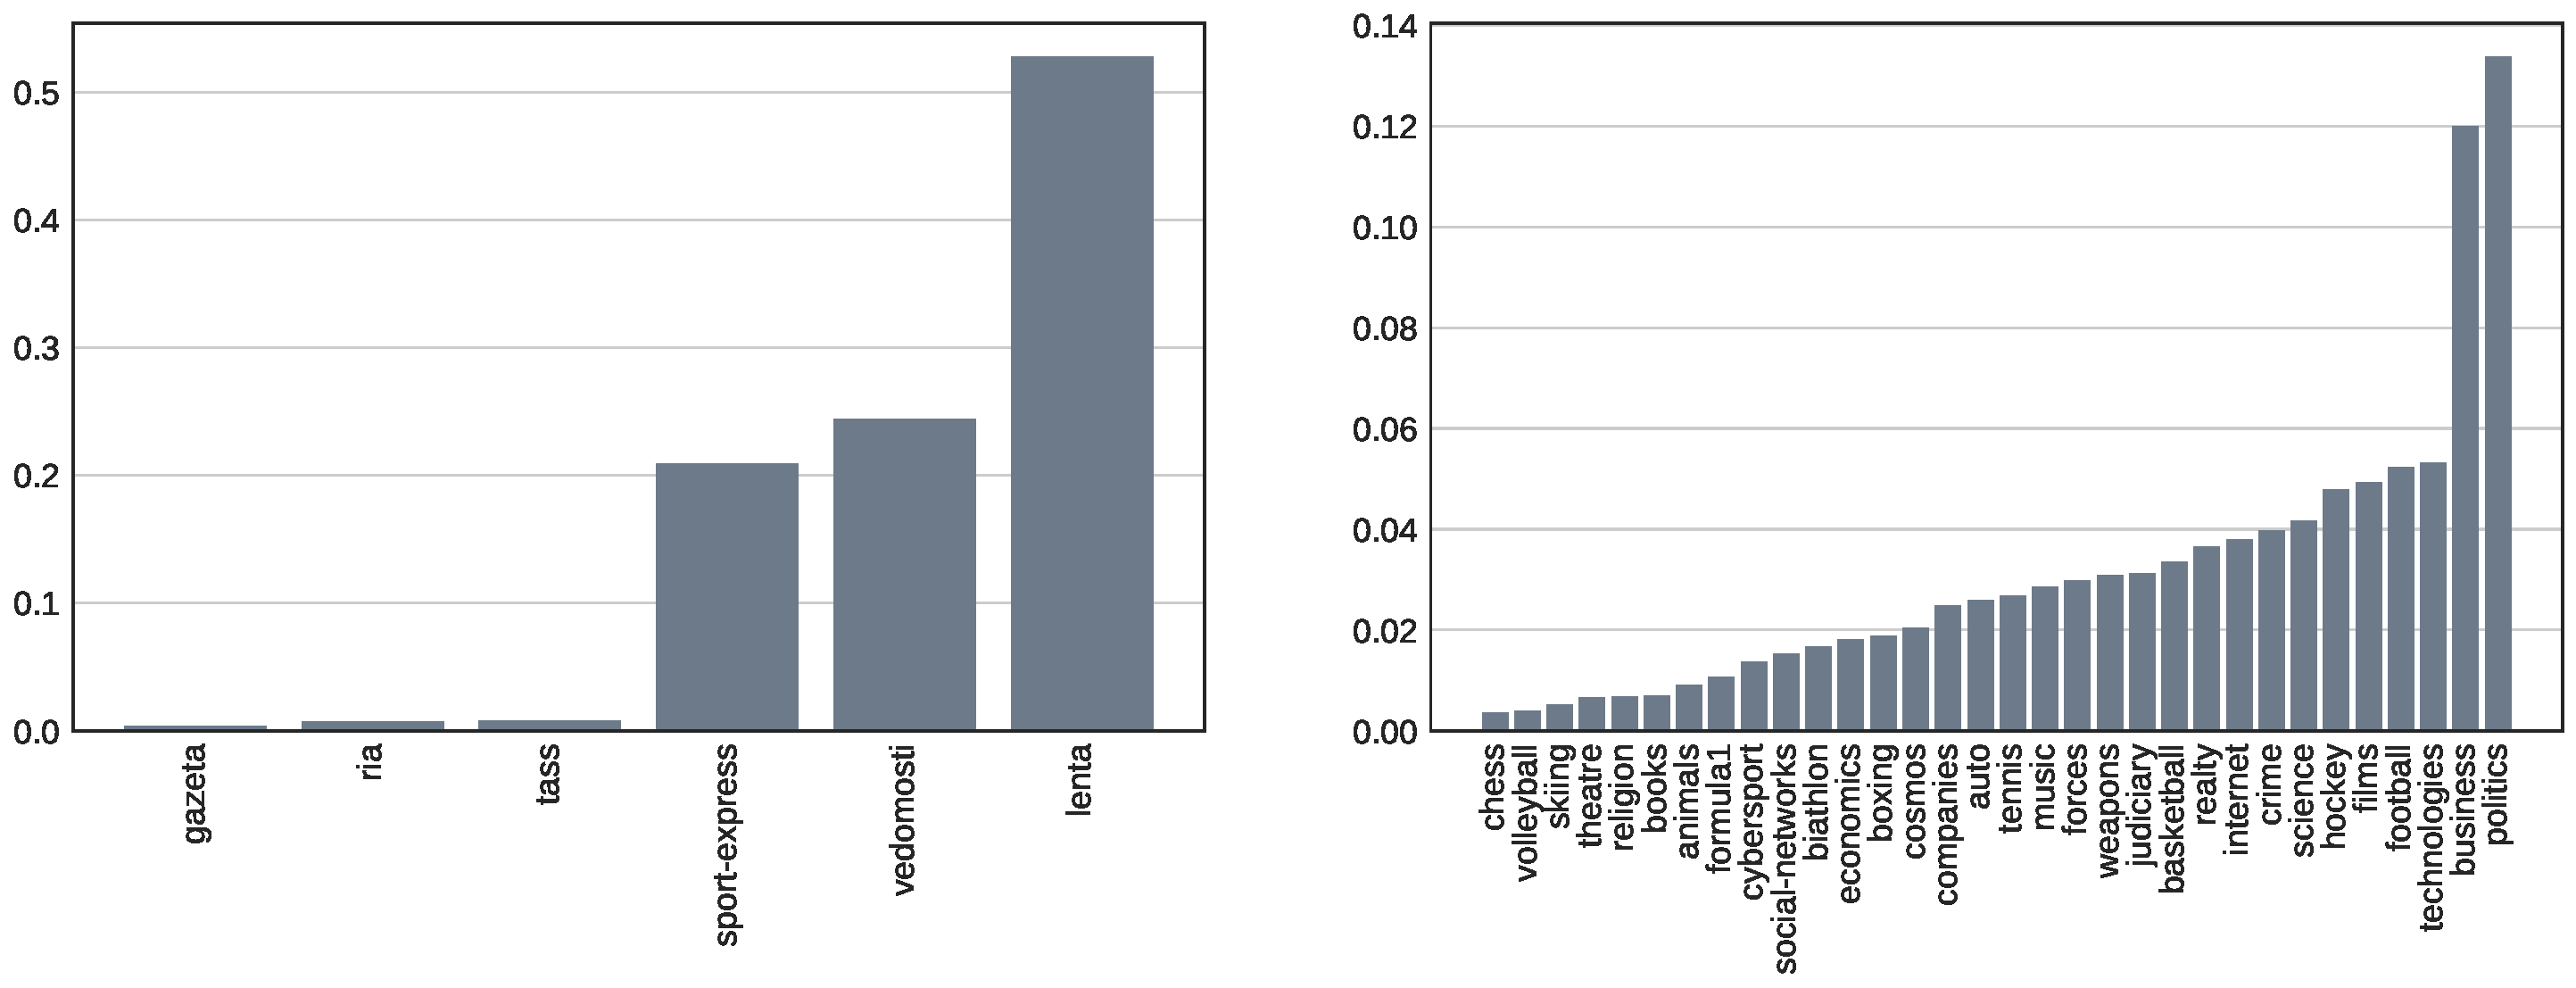
\includegraphics[scale=0.35]{datadistr}
	\caption{Распределение тегов и источников в датасете статей для обучения TF-IDF векторизатора.}
	\label{datadistr}
\end{figure}

От объективности данного датасета зависит качество всего сервиса, так как на нём обучается векторизатор TF-IDF, на котором основан алгоритм кластеризации, а от него, в свою очередь, суммаризация события. Для проверки валидности данных и обученного векторизатора реализован классификатор SVM (support vector machine).

SVM методы классификации используют операции линейной алгебры при работе с векторизованым текстом, при обучении <<пытаясь>> разделить многомерное пространство так, чтобы максимальное количество точек  (векторов) одного и того же класса одного класса находилось в одной части пространства. Это можно достичь с помощью перехода к $n+1$-мерному пространству, как условно показано на рис. \ref{svm_cond}.

\begin{figure}[h!]
	\centering
	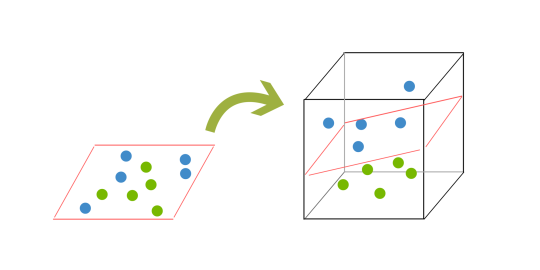
\includegraphics[scale=0.6]{svm_cond}
	\caption{Явное разделение данных на два класса при переходе в пространство более высокой размерности}
	\label{svm_cond}
\end{figure}

SVM классификаторы очень популярный инструмент в NLP задачах, поэтому существует множество реализаций с полезными функциями. Мы использовали его модификацию \verb+SGDClassifier+, которая оптимизирует параметры с помощью градиентного спуска.

Проверка валидности состоит в эмпирической оценке признаков классов~--- это самые <<весомые>> слова, больше всего влияющие на принадлежность к конкретному классу. При изучении слов-признаков из таблицы \ref{word_feachers} видно: слова-признаки и слова-классы связаны по смыслу и, в некоторых случаях, являются синонимами, что свидетельствует о корректности данных и векторизатора. Метрики качества классификаторы тоже поддтверждают правильность датасета: $\text{Accuracy} = 0,8687$, $\text{F1 score} = 0,8711$, матрица ошибок представлена в приложении на рис. \ref{svm_matrix}.

\begin{table}[h]
	\caption{Слова-признаки для собранного датасета.}
	\resizebox{\textwidth}{!}{%
		\begin{tabular}{r|cccccccc}
			\textbf{animals}         &               жить &          вольер &             хозяин &              животный &               зоопарк &        питомец &           кличка &        животное \\
			\textbf{auto}            &          авторынок &           осаго &      автомобильный &     автопроизводитель &              автопром &          камаз &          автоваз &      автомобиль \\
			\textbf{basketball}      &                рфб &      евробаскет &          центровой &          кубок европа &             баскетбол &   баскетболист &         евролига &             нба \\
			\textbf{biathlon}        &           эстафета &    биатлонистка &            шипулин &                   сбр &            хохфильцен &        биатлон &              ibu &      биатлонист \\
			\textbf{books}           &         библиотека &    произведение &       писательница &                 роман &                 книга &   литературный &             поэт &        писатель \\
			\textbf{boxing}          &              алоян &          лебзяк &                мма &              поединок &              поветкин &            бой &             бокс &          боксер \\
			\textbf{business}        &   россельхознадзор &            fifa &                ржд &               газпром &           туроператор &        formula &         ритейлер &             оао \\
			\textbf{chess}           &            карякин &       шахматист &           карякина &                магнус &               шахматы &        карлсен &              фид &       шахматный \\
			\textbf{companies}       &  тысяча автомобиль &        компания &  миллиард кубометр &              миллиард &                тысяча &  процент акция &         ретейлер &         процент \\
			\textbf{cosmos}          &          космонавт &         светить &           прогресс &             вселенная &                космос &     астрофизик &             марс &       астронавт \\
			\textbf{crime}           &          грабитель &         изымать &        группировка &               полиция &               убивать &         летний &       преступник &          тюрьма \\
			\textbf{cybersport}      &             gaming &            team &              valve &           киберфутбол &                  dota &     киберспорт &  киберспортивный &  киберспортсмен \\
			\textbf{economics}       &               мрот &          греция &             бюджет &                пенсия &                   ввп &         минфин &        экономика &        инфляция \\
			\textbf{films}           &         мультфильм &          сериал &            актриса &                  кино &               картина &       режиссер &            актер &           фильм \\
			\textbf{football}        &               поле &         стадион &         нападающий &              матч тур &                  фифа &           уефа &        футболист &    полузащитник \\
			\textbf{forces}          &       развертывать &      выполнение &     военнослужащий &               военный &                 шойгу &        генштаб &       конашенков &      минобороны \\
			\textbf{formula1}        &              манор &      цитировать &               рено &               феррари &              макларен &          пилот &         мерседес &         формула \\
			\textbf{hockey}          &           авангард &             ска &              шайба &            нападающий &                хоккей &       хоккеист &              нхл &             кхл \\
			\textbf{internet}        &          википедия &          сервис &             ресурс &               youtube &                  сайт &          хакер &           блогер &        интернет \\
			\textbf{judiciary}       &             стража &          статья &       арестовывать &               колония &  следственный комитет &      следствие &              скр &  комитет россия \\
			\textbf{music}           &         композитор &     евровидение &              песня &                 певец &               концерт &         альбом &           певица &        музыкант \\
			\textbf{politics}        &              лидер &          кремль &      парламентарий &                партия &               депутат &        госдума &            глава &             мид \\
			\textbf{realty}          &             объект &    строительный &           жилищный &         строительство &                   жкх &        ипотека &            жилье &    недвижимость \\
			\textbf{religion}        &          монастырь &           собор &          церковный &                муфтий &                святой &       христиан &       митрополит &        патриарх \\
			\textbf{science}         &        университет &          журнал &          математик &                 физик &               научный &       археолог &    исследователь &          ученый \\
			\textbf{skiing}          &             вяльбе &          нортуг &             лыжник &                   fis &                легков &         йохауг &            лахти &         устюгов \\
			\textbf{social-networks} &          некоторые &            юзер &           facebook &               twitter &     пользователь сеть &   пользователь &        вконтакте &         соцсеть \\
			\textbf{technologies}    &          vimpelcom &           apple &           оператор &                  wifi &              говорить &            мтс &            робот &         контакт \\
			\textbf{tennis}          &    кубок федерация &            open &            шарапов &                теннис &                  корт &      теннисист &      теннисистка &     кубок дэвис \\
			\textbf{theatre}         &         росгосцирк &        цирковой &              балет &            постановка &           театральный &         мюзикл &            театр &       спектакль \\
			\textbf{volleyball}      &              факел &         маричев &             алекно &             суперлига &             казанский &      белогорье &      волейболист &        волейбол \\
			\textbf{weapons}         &               jane &  использоваться &       defense news &  министерство оборона &             миллиметр &  миллиметровый &          defense &             тип \\
		\end{tabular}
		}
	\label{word_feachers}
\end{table}


\section{Анализ текста}
\subsection{Нормализация}

Текст на естественном языке содержит много избыточных элементов, без которых его смысл не изменится. Чаще всего они действуют как <<шум>>, так как встречается равномерно по всему корпусу языка. Подобными элементами почти всегда выступают союзы, предлоги, части слов, отвечающие за форму. Кроме того, существуют разные способы написания одних и тех же объектов, например, числительные можно написать цифрами. При решении любой задачи в NLP текст нормализуют, то есть приводят в общую, более информативную форму, без <<шума>>. Нормализация включает в себя несколько шагов.

При работе с естественной информацией её дискретизуют. Похожий процесс в NLP называется токенизация, он заключается в делении текста на части~--- токены, обычно токен является одним словом. К сожалению, просто делить текст по пробелам не совсем корректно, так как существует множество исключений, например, Великие Луки~--- это один токен, хотя и состоит из двух слов. Если рассматривать это как два токена, то смысл текста будет искажён, что может сказаться на результате и на качестве решения задачи. Для токенизации удобно использовать регулярные выражения.

В данном проекте используется два токенизатора: простое деление на слова при обработке текста для TF-IDF и Punkt токенизатор для деления статей на предложения при суммаризации. Последний использует корпус для обучение без учителя, <<выучивая>> последовательности, с которых начинаются предложения, что помогает работать с нелитературными данными, например, сообщениями в соц. сетях, где предложения часто начинаются с маленькой буквы.

Следующий шаг нормализации~--- удаление стоп-слов. Стоп-слова примерно одинаково распределены по всему корпусу языка. В русском языке ими являются многие служебные части (союзы, междометия, предлоги).

Для однозначной идентификации слова его приводят к начальной форме. Данный процесс называется лемматизация, а начальная форма~--- лемма. Для лемматизации недостаточно использовать только словарь, потому что существует огромное количество неологизмов, подчиняющимся тем же морфологическим правилам при образовании форм. Хорошие лемматайзеры проводят полный морфологический парсинг, при котором слова делятся на морфемы: стемы (самые осмысленные части) и афиксы (придают дополнительное значение слову) \cite{c2}. Более простая версия морфологического анализа~--- стемминг, использующий определённые правила для извлечения основы слова.% https://web.stanford.edu/~jurafsky/slp3/2.pdf

Мы используем лемматизатор MyStem, предоставляющий универсальный для многих языков алгоритм морфологического разбора, использующийся в популярном поисковом движке.
%https://cache-mskm910.cdn.yandex.net/download.yandex.ru/company/iseg-las-vegas.pdf

При обработке данных перед векторизаций последовательно выполняются следующие операции:
\begin{enumerate}
	\item приведение текста в нижний регистр;
	\item удаление символов пунктуации;
	\item удаление стоп-слов.
	\item лемматизация каждого слова с помощью Python библиотеки MyStem.
\end{enumerate}
 Примеры предложений после данных действий представлен в таблице. \ref{exa}.


\begin{table}[h!]
	\centering
	\caption{Примеры нормализации текста}
	\resizebox{\textwidth}{!}{%
		\begin{tabular}{|l|l|}
			\hline
			Оригинал  & Нормализация \\ \hline\hline
			\makecell[l]{Однако когда их проверили на восприятие\\ концепций и идей, оказалось, что те, \\кто писал от руки, понимают пройденный \\материал лучше однокашников.} & \makecell[l]{однако когда они проверять на восприятие \\концепция идея оказываться что тот \\кто писать от рука понимать проходить\\ материал хорошо однокашник}
			\\ \hline
			\makecell[l]{Лингвистическую относительность упоминали\\ в своих сочинениях немецкие философы\\ еще в конце XVIII – начале XIX века, \\но известность гипотеза получила\\ именно благодаря Уорфу.} & \makecell[l]{лингвистический относительность упоминать \\свой сочинение немецкий философ \\еще конец xviii – начало xix век \\но известность гипотеза получать\\ именно благодаря уорфу} \\ \hline
		\end{tabular}
	}
	\label{exa}
\end{table}


\subsection{Векторизация}

TF-IDF \cite{doi:10.1108/eb026526} --- статистическая мера, используемая для оценки важности слова в любом контексте, основанная на его встречаемости в документе. Чем реже слово появляется в документе, тем выше его TF-IDF вес.

TF-IDF --- это произведение двух статистик: TF (term frequency) и IDF (inverse 
document frequency). 

Существует несколько способов подсчёта TF-IDF, в данной работе использовался следующий:
$$
\text{tf}(t, d) = \cfrac{n_t}{\sum_{k} n_k},
$$
где $n_{t}$ есть число вхождений слова $t$ в документ, а $\sum_{k} n_k$ --- общее число слов в данном документе.

$$
\text{idf}(t, D) = \log{ \cfrac{|D|}{|\{ d_i \in D \mid t \in d_i \}|}},
$$
где $|D|$ --- число документов в корпусе, $|\{ d_i \in D \mid t \in d_i \}|$ — число документов из корпуса $D$, в которых встречается 
$t$ (когда $n_{t} \neq 0$).

Таким образом, мера TF-IDF является произведением двух сомножителей:
$$
\text{TF-IDF}(t, d, D) = \text{tf}(t, d) \cdot \text{idf}(t, D).
$$

Признаковым описанием одного объекта $d \in D$ будет вектор
$$
\big(\text{TF-IDF}(t,d,D)\big)_{t\in V},
$$
где $V$ --- словарь всех слов, встречающихся в корпусе $D$.

Обучение модели заключается в подсчёте веса каждого уникального слова в каждом документе.
\subsection{Кластеризация}
Представленные в виде векторов статьи можно кластеризовать алгоритмом k-means. Если подобрать оптимальные параметры количества кластеров и максимального расстояния от центра кластера, после которого статья удаляется из кластера, то статьи в одном кластере будут об одном событии \cite{km}.

\subsection{Суммаризация}
\subsubsection{SumBasic}
\subsubsection{DivRank}


\section{Реализация сервиса}
\subsection{Архитектура и транспорт данных}
\subsection{Особенности реализации компонентов анализа}
\subsubsection{Система сбора данных}

{\LARGE ПЕРЕПИСАТЬ, ВСЁ УЖЕ НЕ ТАК}
Система сбора данных представляет собой коллекцию парсеров сайтов российских СМИ, основанные на одном подходе и имеющие одинаковый интерфейс. Пример использования представлен на рис. \ref{example}.

В общей архитектуре сервиса система является обособленным фоновым процессом, собирающим раз в некоторое время новые статьи, поэтому нет необходимости постоянно поддерживать строгие ограничения к скорости парсинга. Но эту же систему можно использовать для относительно быстрого сбора собственного датасета. Кроме того, при инициализации сервиса понадобится получить новости за последние несколько часов, чтобы сформировать актуальные кластера. Парсинг множества статей можно ускорить в несколько раз, обрабатывая их параллельно.

Чтобы понять, как реализовать универсальную систему, с возможностью быстрого добавления поддержки нового ресурса, достаточно взглянуть на сайты русскоязычных медиа-ресурсов. Многие сильно отличаются друг от друга внешне, но у всех присутствует следующая логика: существуют страницы со списком новостей в хронологическом порядке, которые либо агрегированы по дням (Lenta.ru, Gazeta.ru, vedomosti.ru), либо используют параметр offset, указывающий с какой статьи начинать страницу (novayagazeta.ru, tass.ru, meduza.io). Первый вариант пагинации удобнее, потому что позволяет просто получить новости за любой заданный интервал времени. Во втором случае можно использовать бинарный поиск по страницам, но это не реализовано, так как новости всегда нужны с текущего момента.
Большинство СМИ отдают данные в HTML формате и только лишь малая часть использует API в JSON формате.

Так как система обособлена, то писать её можно на любом языке, а взаимодействовать с сервисом через внешнее хранилище, но для удобства выбран \texttt{Python 3}, с использованием дополнительных библиотек: \texttt{BeautifulSoup} для парсинга HTML и \texttt{requests} для выполнения HTTP запросов. Так как Питон имеет ограничение на потоки из-за GIL, то чтобы обеспечить параллелизм, позволяющий с увеличением количества процессорных ядер ускорять обработку множества статей, используется модуль \texttt{multiprocessing}.

\begin{figure}
	\centering
	\begin{minted}[fontsize=\small]{python}
	from parsers import Gazeta, Tass, Lenta, Vedomosti, Novaya
	import datetime
	
	parsers = [
	Gazeta(procs=4), # Number of processes used
	Tass(),
	Lenta(),
	Vedomosti(),
	Novaya(procs=4)
	]
	until_time = datetime.datetime.now() - datetime.timedelta(hours=4)
	for parser in parsers:
	print(parser.id)
	for n in parser.get_news(until_time=until_time):
	print(n['title'])
	\end{minted}
	\caption{Пример использования для получения всех новостей за последние 4 часа.}
	\label{example}
\end{figure}

Главной частью системы является класс \texttt{BaseParser}, инкапсулирующий сетевые запросы, работу по синхронизации процессов и передаче данных между ними. В целом, логика межпроцессного взаимодействия системы достаточно тривиальная и находится в методе \texttt{get\_news} (рис. \ref{getnews}): процесс-предок запускает процессы-потомки и начинает заполнять очередь задач ссылками на статьи, в этот момент дочерние процессы уже разбирают ссылки из очереди и обрабатывают их. В качестве очереди задач выступает класс \texttt{multiprocessing.Queue}, который комбинирует межпроцессное взаимодействие через pipe и разделяемые блокировки. Благодаря модулю pickle очередь может передавать сложные объекты и часто применяется в подобных случаях. 

После того, как основной процесс закончил парсинг страниц и отправил все задачи в очередь, он меняет значение переменной \texttt{sync\_flag}, которая находится в общем для процессов сегменте памяти (Shared memory), если значение меняется, процессы-потомки понимают, что после опустошения очереди можно больше её не <<слушать>>.

\begin{figure}
	\centering
	\begin{minted}[fontsize=\small]{python}
	def get_news(self, start_time=None, until_time=None,
	news_count=None, topic_filter=None):
	. . .
	
	Q_urls = Queue(0) # News urls and for deeper parsing 
	Q_out = Queue(0) # Results of parsing
	sync_flag = Value('i', 1) # Flag to stop processes
	
	workers = []
	# Getting news by url in proceses
	for _ in range(procs):
	workers.append(Process(target=self._process_news,
	args=(Q_urls, Q_out, sync_flag, topic_filter)))
	workers[-1].start()
	# Parsing pages with urls ("Лента новостей") and putting them to Q_urls
	self.parse_pages(Q_urls, sync_flag, start_time, 
	until_time, news_count, topic_filter)
	# Clearing output queue while processes still working
	# Probably significantly slowing down other workers, need to fix it
	out = []
	self._listen_queue(workers, Q_out, out)
	. . .
	\end{minted}
	\caption{Часть кода класса \texttt{BaseParser}.}
	\label{getnews}
\end{figure}

Результаты выполненных задач не принято передавать родительскому процессу, но в данном случае это было сделано для удобства интерфейса с помощью второй очереди. После смены значения общего флага предок начинает <<слушать>> очередь и ждать результатов. Такой подход крайне нежелателен, так как результат в разы больше параметров самой задачи (из-за текста статьи), и при большом количестве обработанных новостей все процессы-потомки останутся висеть в простое, пока предок будет извлекать из очереди результаты. На небольших объёмах это незаметно, но запускать такое на 64 ядерном процессоре в 64 процесса с целью выкачать новости за несколько лет не стоит.

Описанная проблема будет решена заменой Pipe-очереди на базу данных в оперативной памяти (in-memory database), например, на Redis. Можно решить её и с использованием Shared memory, но это гораздо сложнее, так как объекты Питона придётся сериализовывать для хранения и десериализовывать для использования вручную.

Чтобы создать новый парсер необходимо наследоваться от \texttt{BaseParser}, вызвать родительский конструктор с параметрами: название парсера, URL-префикс любой новости ресурса, URL-префикс ленты новостей, дефолтное количество процессов. Определить следующие методы:
\begin{itemize}
	\item \texttt{\_get\_news\_list(self, content)}~--- возвращает список списков с необработанными параметрами новости, используя контент (HTML или JSON) ленты новостей.
	\item \texttt{\_get\_news\_params\_in\_page(self, news)}~--- возвращает \texttt{tuple} с параметрами статьи, используя элемент списка из предыдущего метода. URL и дата (в \texttt{datetime} объекте) должны быть первыми в списке параметров (\texttt{dict} не используется в данном случае в попытке выиграть время и место на pickle-запаковке объекта).
	\item \texttt{\_parse\_news(self, news\_params)}~--- возвращает \texttt{dict} с новостью, например, \mintinline[fontsize=\small]{python}/{'title': title, 'url': url, 'text': text, 'topic': topic, 'date': date}/.
	\item \texttt{\_page\_url(self)}~--- возвращает URL текущей страницы.
	\item \texttt{\_next\_page\_url(self)}~--- <<переворачивает>> страницу и возвращает \texttt{\_page\_url}.
\end{itemize}





\begin{figure}
	\centering
	\begin{minted}[fontsize=\small]{python}
	from nltk.corpus import stopwords
	from pymystem3 import Mystem; mystem = Mystem()
	import string
	from stop_words import get_stop_words
	
	STOP_WORDS = (set(stopwords.words('russian')) | set(stopwords.words('english')) | 
	set(get_stop_words('ru')) | set(get_stop_words('en')))
	
	def get_word_normal_form(word):
	return ''.join(mystem.lemmatize(word)).strip().replace('ё', 'е').strip('-')
	
	def lemmatize_words(text):
	text = text.lower()
	text = ''.join([i for i in text if ( i not in string.punctuation )])
	res = []
	for word in text.split():
	norm_form = get_word_normal_form(word)
	if len(norm_form) > 2 and norm_form not in STOP_WORDS:
	res.append(norm_form)
	return ' '.join(res)
	\end{minted}
	\caption{Простая функция нормализации.}
	\label{norm}
\end{figure}




\subsubsection{Модуль нормализации}
\subsubsection{TF-IDF и SVM}
\subsubsection{KMeans}
\subsubsection{SumBasic}
\subsubsection{DivRank}

\subsection{Инфраструктура и развёртка}

\section{Оценка решений}
\section{Заключение}


\bibliography{biblio} % Список литературы

\section*{Приложение}
\begin{figure}[h!]
	\centering
	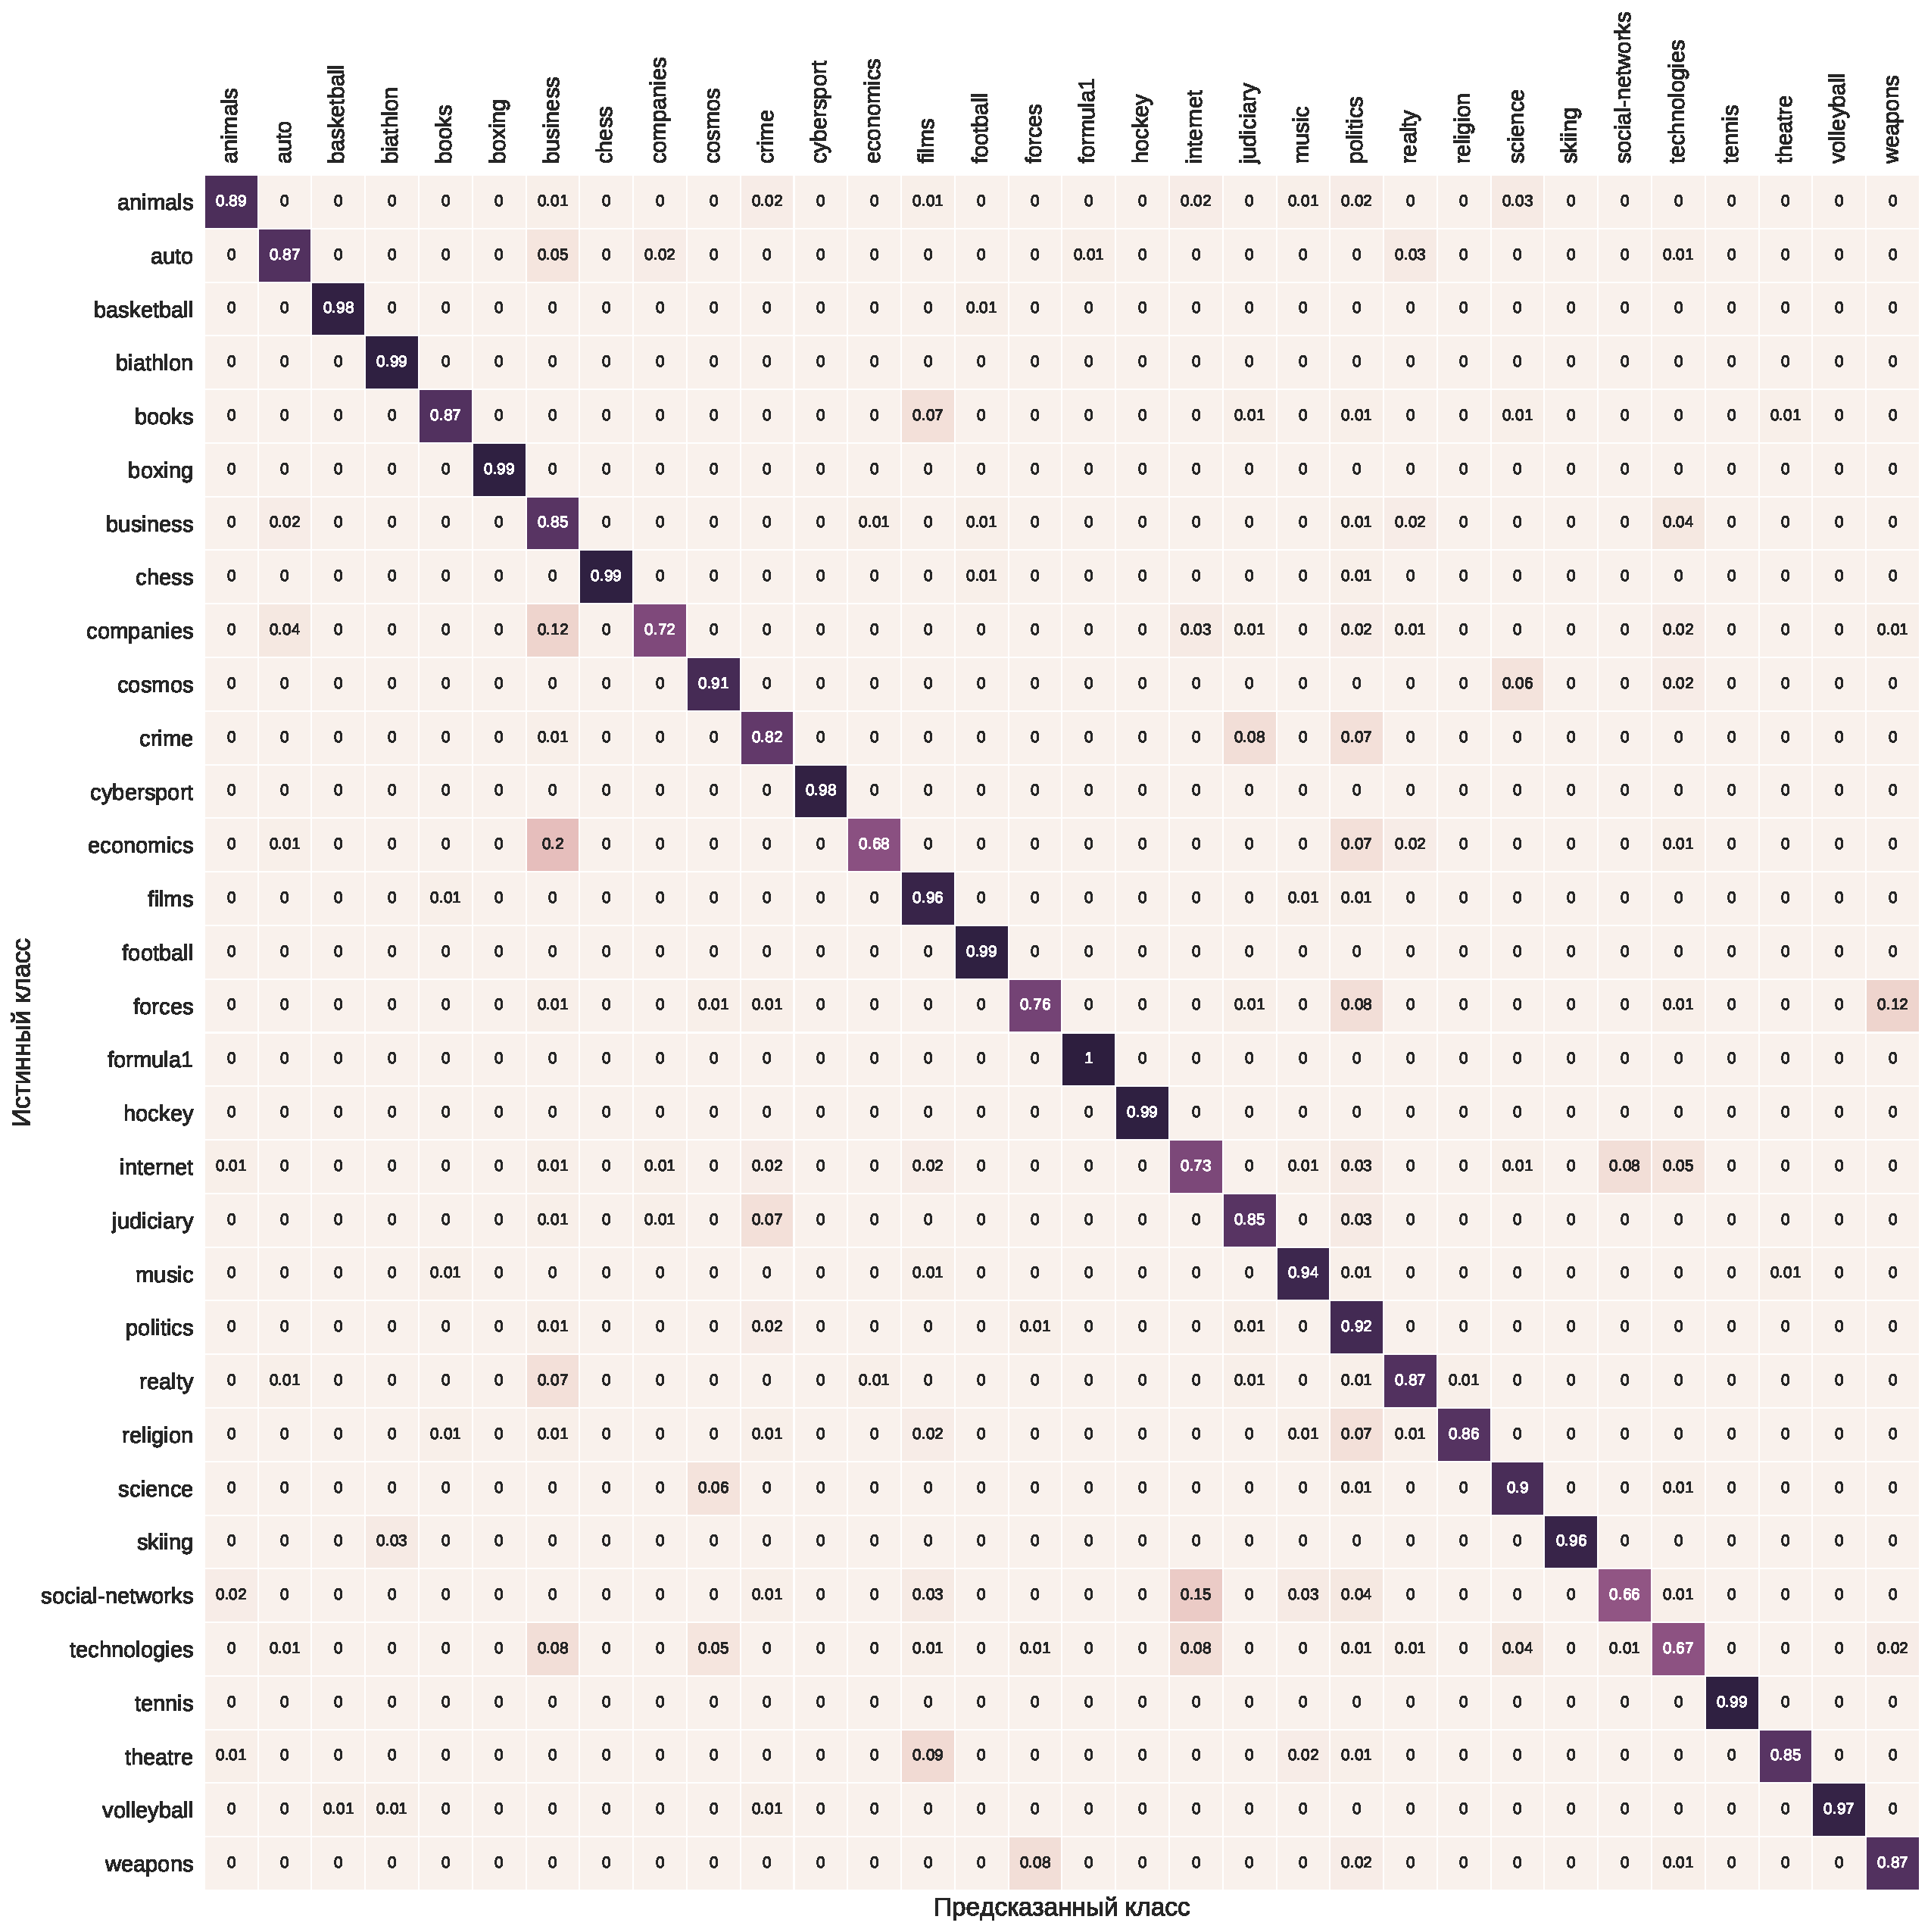
\includegraphics[width=0.95\textwidth]{svm_matrix}
	\caption{Ошибки классификатора SVM}
	\label{svm_matrix}
\end{figure}

\end{document}